\documentclass{article}

% Encodings, page setup, paragraph formatting, font
\usepackage[top=0.9in, bottom=1in, left=1.5in, right=1.5in]{geometry}
\usepackage[icelandic]{babel}
\usepackage[T1]{fontenc}
\usepackage[sc]{mathpazo}
\usepackage[parfill]{parskip}
\usepackage{cancel}
\usepackage{comment}
% Tables and lists
\usepackage{booktabs,tabularx}
\usepackage{multirow}
\usepackage{enumerate}
\usepackage{adjustbox}
\usepackage{multicol}
\usepackage{enumitem}
\usepackage{xcolor}
% Math
\usepackage{amsmath, amsfonts, amssymb, amsthm}
% Graphics
\usepackage{graphicx}
\usepackage{forest}
\usepackage{tikz}
\usetikzlibrary{positioning, shapes, arrows.meta}
% Code environment
\usepackage{listingsutf8}
\definecolor{commentcolor}{RGB}{0, 128, 0} % Grænn
\definecolor{keywordcolor}{RGB}{0, 0, 255}   % Blár
\definecolor{stringcolor}{RGB}{163, 21, 21}      % Dökkrauður
\definecolor{numbercolor}{RGB}{128, 0, 128}      % Fjólublár
\definecolor{identifiercolor}{RGB}{0, 0, 0}      % Svartur

\lstset{
    language=Java,
    basicstyle=\ttfamily,
    keywordstyle=\color{keywordcolor}\bfseries,
    commentstyle=\color{commentcolor},
    identifierstyle=\color{identifiercolor},
    stringstyle=\color{stringcolor},   
    showstringspaces=false,
    numbers=left,
    numberstyle=\tiny\color{gray},
    tabsize=2,
    breaklines=true,
    columns=fullflexible,
    keepspaces=true,
    inputencoding=utf8, 
    extendedchars=true,  
    literate=
        {á}{{\'a}}1
        {ð}{{\dh}}1
        {é}{{\'e}}1
        {í}{{\'i}}1
        {ó}{{\'o}}1
        {ú}{{\'u}}1
        {ý}{{\'y}}1
        {þ}{{\th}}1
        {æ}{{\ae}}1
        {ö}{{\"o}}1
        {Á}{{\'A}}1
        {Ð}{{\DH}}1
        {É}{{\'E}}1
        {Í}{{\'I}}1
        {Ó}{{\'O}}1
        {Ú}{{\'U}}1
        {Ý}{{\'Y}}1
        {Þ}{{\TH}}1
        {Æ}{{\AE}}1
        {Ö}{{\"O}}1,
}

% Restin af forskriftinni
\usepackage[pdftex,bookmarks=true,colorlinks=true,pdfauthor={Hafsteinn Einarsson},linkcolor=blue,urlcolor=blue]{hyperref}

% Hyphenation
\hyphenpenalty=5000
% Page and section numbering
\setcounter{secnumdepth}{-1} 
\pagenumbering{gobble}

\title{Tölvutækni og forritun Lokapróf}
\author{brj46 }
\date{Nóvember 2024}

\begin{document}

\maketitle

\newpage

\section{Tekið frá Tuma}

\subsection{assembly}



\subsection{Uppbrot Gistis}

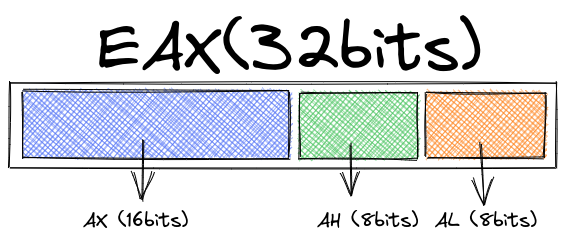
\includegraphics[scale = 0.8]{gistabrot.excalidraw.png}

\subsection{algengar skipanir}

\begin{tabularx}{\textwidth}{|l|l|X|}
\hline
    \textbf{skipun} & \textbf{argument} & \textbf{lýsing} \\ \hline
    mov & x, y & færir úr x yfir í y, sjá conditional move fyrir neðan\\ \hline 
    push & x & ýtir x á hlaða og eftir að hækka \text{\%ESP} um sizeof(x) bæti og sett þar inn \\ \hline
    pop & x & skilar síðasta gildi sem var sett á hlaðann inn í x \\ \hline
    lea & (x), y & lea, betur þekkt sem leaq er notað til að framkvæma reikning (x) og setja útkomu inn í y \\ \hline
    (x,y) & &skilar útkomu úr reikningi x + y \\ \hline
    0,(,x,y) & & skilar útkomu úr reikningi x * y \\ \hline
    (x,y,z) & & skilar útkomu úr reikningi x + y * z \\ \hline
    2(x, y, z) & & skilar útkomu úr reikningi (2 + (x + y * z)) \\ \hline
    sar & x, y & hliðrar y um x bita til hægri, basically heiltöludeiling með x\\ \hline
    sal & x, y & næstum eins og sar nema til vinstri, núna með margföldun með $2^x$ \\ \hline
    sub & x,y & dregur y frá x \\ \hline
    inc/dec & x & hækkar/lækkar gildi x um 1\\ \hline
\end{tabularx}

ath. \textbf{SHL} og \textbf{SAL} gera það sama en \textbf{SHR} virkar ekki með signed int eins og \textbf{SAR}

\subsection{Algeng mynstur}





\begin{tabularx}{\textwidth}{|l||X|}

 \textbf{ mynstur } &  \textbf{skýring} \\ \hline
    testl \%edi, \%edi & logical andað \textbf{edi} við \textbf{edi} þannig ef $edi <= 0$ er hægt að cmove eða jc í samræmi við það \\ \hline
    cmove $\$5$, \text{\%eax} & færðu 5 inn í eax ef z-flaggið er sett sem 1 þ.e. ef edi er tómt \\ \hline
    leal 0(\text{\%rdi, \%rdi, 4}) & margfaldar \text{\%rdi} með 5, $(x+4 *x)$ \\ \hline
\end{tabularx}
\newpage

\subsection{conditional codes}


þessir kóðar fara a endann á cmov skipunum þ.e. cmov-- í línu eftir að eitthvað er testað eins og í dæmi 

\begin{verbatim}
    testb   $7, %dl
    cmove   $1, %rax
\end{verbatim}

Þetta er pínu fucked dæmi því e flaggið í cmove stendur fyrir equal nema hvað við erum actually að athuga hvort útkomugildið sé 0, þ.e. að enginn af neðstu 3 bitunum sé 1, þá er gott að muna að e er jafngilt z

þessi koði færir 1 inn í \text{\%rax} ef neðstu þrír bitar \text{\%dl} eru ekki 111

\begin{tabular}{|c|c|}
\hline
     \textbf{cc}& \textbf{condition}  \\ \hline
    o  & overflow \\ \hline
    no & no overflow \\ \hline
    b, nae & below, not above or equal \\ \hline
    nb, ae & not below, above or equal \\ \hline
    e, z & equal(zero) \\ \hline
    ne, nz & not equal, (not zero) \\ \hline
    na, be & not above, below or equal \\ \hline
    a, nbe & above, not below or equal \\ \hline
    s & sign \\ \hline
    ns & no sign \\ \hline
    p & parity \\ \hline
    np & no parity \\\hline
    l, nge & less, not greater than or equal \\ \hline
    nl & not less, greater than or equal \\ \hline
    ng, le & not greater, less than or equal\\ \hline
    g, nle & greater, not less than or equal \\ \hline
\end{tabular}

\subsection{minnissvæði}


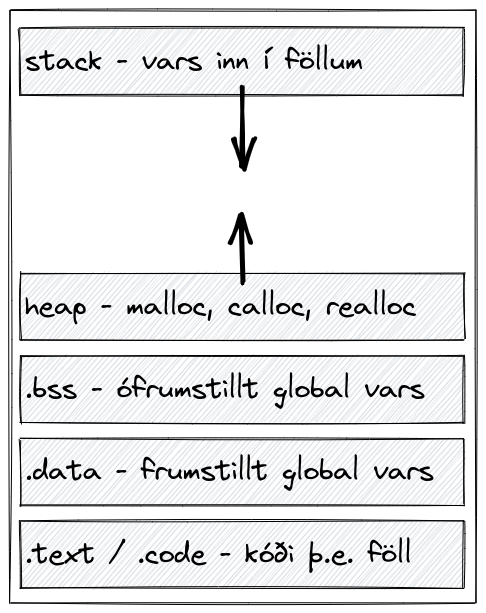
\includegraphics[scale = 0.4]{minni.excalidraw.png}

ath. global breytur sem eru skilgreindar sem 0 eða NULL eru líka í .bss
\newpage

\subsection{Sýndarminni}
\begin{itemize}
    \item sýndarvistföng: a bitar
    \item raunvistföng: b bitar
    \item síðustærð: c bæti
    \item TLB: d vítt, e sæti
    \item fjöldi mengha: f
\end{itemize}

fjöldi mengja er reiknað $\frac{e}{d} = f$

við erum með sýndarvistfang sem er 16 bitar sem skiptast í 4 mengi
þá er \textbf{VPN}$\frac{3}{4} \times 16$ bitar og \textbf{VPO} 4 bitar

\textbf{TBLT} og \textbf{TLBI} eru skipting á \textbf{VPN} og \textbf{TBLT} restin raunvistföngin eru jafn löng og \textbf{TLBT} og skipt niður í tvo hluta \textbf{PPN} og \textbf{PPO}, sem er jafn stór og \textbf{VPO}(í þessu tilfelli 4 bitar)

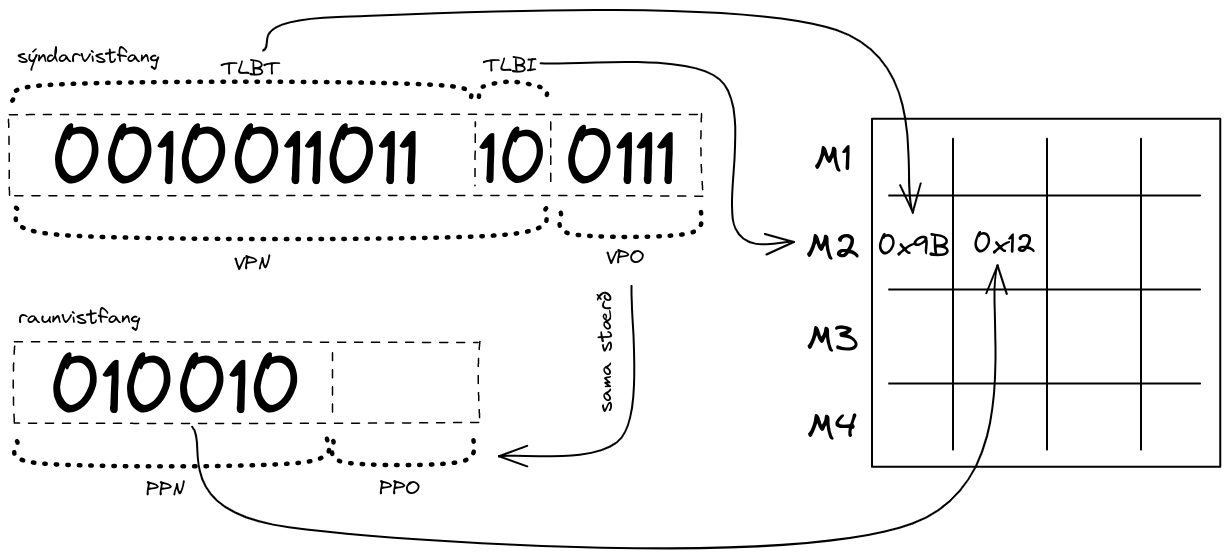
\includegraphics[scale = 0.2]{syndarminni.excalidraw.png}

annap dæmi, við erum með sýndarminni sem er 4kb að stærð, 4-vítt, E, og með 16 mengi, S, svo útfrá þessum tölum finnum við línustærð, B, með reikningnum $\frac{4096}{16 \times 4} = 64$ skiptum þessu nu upp fyrir 32-bita vistfang:

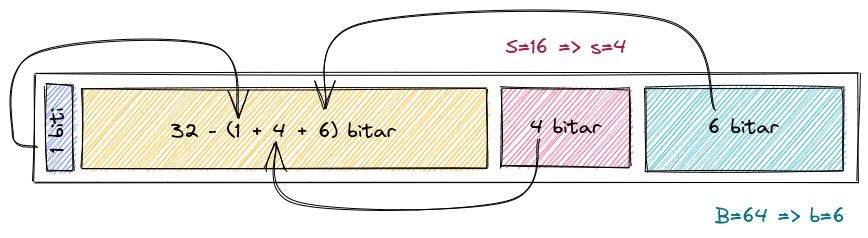
\includegraphics[scale = 0.5]{skipting.excalidraw.png}

\subsection{klukkutifsformúla}


$a + s \times r = m$
\begin{itemize}
    \item aðgangstími = a(tif)
    \item smellahlutfall = s(hlutfall)
    \item smellarefsing = r (tif)
    \item meðalaðgangstími = m (tif)
\end{itemize}

dæmi:
\begin{itemize}
    \item \text{97\%} smellahlutfall, $1 + 0.03 \times 100 = 4$
    \item \text{99\%} smellahlutfall, $1 + 0.01 \times 100 = 2$
\end{itemize}


\newpage
\section{Vika 1}
\large{\textbf{Kynning, Linux, C}}

\subsection{Heimadæmi spurningar}

\subsubsection{1 og 2}
kennslu aðferðir

\subsubsection{3}
Skoðið sýnidæmin á glæru 16 í fyrirlestri 1 (þ.e. $50000 * 50000$ fyrir int og $1e20 +
(-1e20 + 3.14)$ fyrir float).
\begin{itemize}
    \item[a]. Skrifið stutt forrit í Java sem prentar út niðurstöðuna úr þessum útreikningunum
(athugið að í Java eru kommutölufastar sjálfkrafa af taginu double. Til að fá
float-fasta þarf að setja f á eftir fastanum, t.d. 3.14f).
\item[b] . Reyndar er gildið 1e20 (þ.e. 1020) óþarflega stórt. Það eru til mun minni gildi
sem valda sömu vandræðum. Finnið lægsta gildi a á 10a sem gefur sömu
niðurstöðu og 1e20 í seinni formúlunni á glæru 16. Sýnið útprentun á því í Java
forriti.
\end{itemize}

\subsubsection{4}
Á glærum 20 og 21 í fyrirlestri 1 er sýnd minnisvilla sem getur komið upp í C forriti.
Útskýrið hvers vegna svona villa myndi ekki koma upp í sambærilegu Java forriti.
Hvaða kostir og gallar eru við það að leyfa möguleika á svona villum í C forritum?

\subsubsection{5}
Setjið upp linux



\newpage
\section{Vika 2}
\large{\textbf{C, Bendar, minni, notkun}}

\newpage
\section{Vika 3}
\large{\textbf{Upplýsingar sem bitar, heiltölur}}

\newpage
\section{Vika 4}
\large{\textbf{Bætaröð, fleytitölur}}

\newpage
\section{Vika 5}
\large{\textbf{Skipulag örgjava, smalamálsforritun}}

\newpage
\section{Vika6}
\large{\textbf{Stýriskipanir og stef í smalamáli}}

\newpage
\section{Vika 7}
\large{\textbf{Gögn og yfirflæði minnis}}

\newpage
\section{Vika 8}
\large{\textbf{Bestun smalamálskóða}}

\newpage
\section{Vika 9}
\large{\textbf{Minnisstigveldi, skyndiminni}}

\newpage
\section{Vika 10}
\large{\textbf{Tenging, keyrsluskrár, forritasöfn}}

\newpage
\section{Vika 11}
\large{\textbf{Frábrigði, ferlastýring}}

\newpage
\section{Vika 12}
\large{\textbf{Sýndarminni}}

\newpage
\section{Vika 13}
\large{\textbf{Minnisúthlutun, ruslasöfnun, minnisvillur}}

\newpage
\section{Vika 14}
\large{\textbf{Samantekt}}


\end{document}
